
%
%  $Description: Author guidelines and sample document in LaTeX 2.09$ 
%
%  $Author: ienne $
%  $Date: 1995/09/15 15:20:59 $
%  $Revision: 1.4 $
%

\documentclass[times, 12pt,twocolumn]{article} 
\usepackage{latex8}
\usepackage{times}
\usepackage{graphicx}
\usepackage{epstopdf}
\usepackage{enumitem}
\usepackage[font=small]{caption}
\usepackage[utf8]{inputenc}
\usepackage{url}
\usepackage{courier}
\usepackage{listings}
%\documentstyle[times,art10,twocolumn,latex8]{article}

%------------------------------------------------------------------------- 
% take the % away on next line to produce the final camera-ready version 
\pagestyle{empty}

%------------------------------------------------------------------------- 
\begin{document}

\title{Randomized Consensus Project Report}

\author{Bogdan Suvar, Daniel Bali, Seckin Savasci\\
Instituto Superior T\'{e}cnico\\
\texttt{\{bogdan.suvar,janos.bali,seckin.savasci\}@tecnico.ulisboa.pt}\\
}
 
\maketitle
\thispagestyle{empty}

\begin{abstract}
   The FLP impossibility states that no deterministic algorithm 
   can solve consensus in an asynchronous system where at least one 
   process can crash. To circumvent this, we can relax the conditions 
   and make a probabilistic algorithm for consensus. This report will 
   give details on our implementation of Randomized Consensus.
\end{abstract}

%------------------------------------------------------------------------- 
\Section{Stack}

\begin{figure}[ht!]
\centering
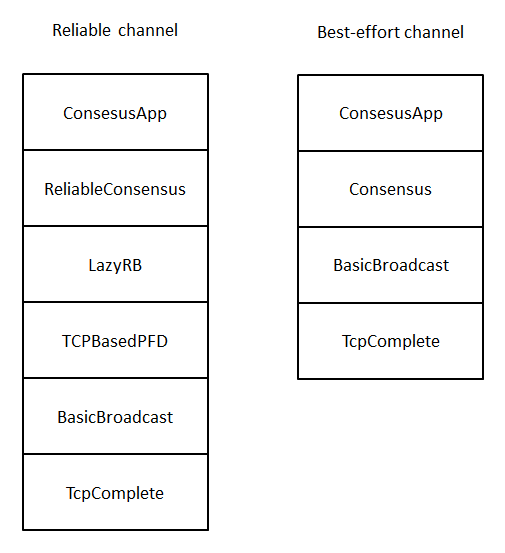
\includegraphics[width=80mm]{stack.png}
\caption{Applia layer stack}
\label{fig:stack}
\end{figure}

Two channels are required according to the Randomized Consensus algorithm. 
For the first phase of the protocol, it is sufficient to use 
\textit{Best-effort Broadcast}. For the final part of the second phase, 
\textit{Reliable Broadcast} is required. For this reason we used two 
separate stacks, which can be seen on figure \ref{fig:stack}.

For the reliable channel, we had to use Lazy Reliable Broadcast on top
of a TCP-based Perfect Failure Detector. The best-effor channel is much simpler, 
only requiring a basic broadcast layer.

The implementation of the randomized consensus algorithm is in the 
\textit{tfsd.consensus} package. \textit{ConsensusLayer} is the layer for the 
session that uses the best-effort channel. \textit{ReliableConsensusLayer} is for 
the reliable channel. ConsensusLayer requires ChannelInit and ProcessInitEvent. 
Above these, it accepts ProposeEvent and SendableEvent.

%------------------------------------------------------------------------- 
\Section{Code}

\begin{figure}[ht!]
\centering
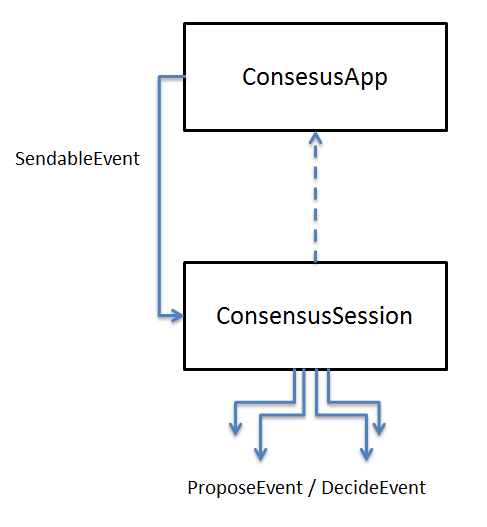
\includegraphics[width=80mm]{arch.png}
\caption{Architecture of the application}
\label{fig:arch}
\end{figure}

This section contains a brief explanation of the code and its connection 
to the randomized consensus algorithm.
 
Figure \ref{fig:arch} shows the basic outline of the architecture for our 
solution. The \textit{ConsensusApp} sends SendableEvents to the ConsensusSession, 
where they are converted to ProposeEvents and broadcasted. When the algorithm 
reaches the end of phase 2, this session notifies the ConsensusApp, which in turn 
sends a SendableEvent to ReliableConsensusApp. This session will then reliably 
broadcast the request to start the decision process.

The main part of the algorithm is implemented in ConsensusSession. 
\textit{handleSendable} is the function responsible for converting SendableEvents 
into ProposeEvents which are then broadcasted.

After a ProposeEvent is received, its parameters are observed. It has three main 
parameters: phase, value and timestamp. The propose event is then processed according 
to its phase.

In phase one, the algorithm waits for a majority. This is handled by 
\textit{handleProposePhase1}. When a majority is reached, we check if the values 
are the same. If they are, we enter phase two with this value - entering means 
we send a new ProposeEvent with the phase set to two. When the values are not the 
same, we enter phase two with the \textit{bottom value}.

Phase two waits for all replies, minus the number of tolerated failures. 
When a quorum is reached, it tries to find f+1 occurences of the same v* value. 
When this is found, it issues a decide.

When a decision could not be made, we restart the algorithm from phase one, with 
a random value from the previously seen proposals. After the restart, the 
queues of the quorums are emptied.

Timestamps are used to differentiate between different proposals. There is a started 
and a decided timestamp. When we see a proposal with a timestamp that is less-than 
or equal to our decided timestamp, we can discard it.

%-------------------------------------------------------------------------

\Section{Running the code}

%-------------------------------------------------------------------------

\Section{Evaluation}

%-------------------------------------------------------------------------

\bibliographystyle{latex8}
\bibliography{latex8}

 
\end{document}
